\section{Theoretical Background} \label{sec:theoretical_background}

This chapter serves the presentation of the most relevant definitions and methods for understanding the l-WWLLT method and its performance.
Each section is summarized by a reference that indicates how the definitions given are used in the method.

First, definitions from Graphtheory are presented. 
These are necessary to understand both the used data and the structures to define the graph similarity measure on them.
Next, different metrics and the basics of the used graph similarity measure are presented.
Thirdly, the already mentioned Weisfeiler-Leman labeling scheme and a hierarchy on the resulting Weisfeiler-Leman labels is defined. 
Both are central in the computation of the graph representations used in the similarity measure.
Next, as indicated in the related work paragraph (in section \ref{subsec:related_work}), graph kernels prove useful to apply and compare the similarity measure.
Thus kernels in general, graph kernels, and important example are introduced.
At last, some terminology to evaluate clustering algorithms and Support Vector Machines is given. 
These are used for the evaluation of the l-WWLLT method.

\subsection{Graph Theory} \label{subsec:def_graphtheory}
	
	The goal of the l-WWLLT method is to define a similarity measure on graphs.
	In order to be able to do so we first define similarity measure on substructures of such graphs.
	This similarity measure is based on a special graph called tree, which is the backbone of the method.	
	Therefore the relevant definitions from the field of Graphtheory are stated in this section.
	
	We define a \textbf{graph}\label{def:Graph} as a tuple $G=(V, E)$, where $V$ denotes a finite set of vertices and $E\subseteq 2^V$ a finite set of edges on $V$. 
	We also write $V(G)$ to refer to the vertices of a graph $G$.
	In this thesis we consider edges to be undirected. 
	That is an \textbf{edge} is a set of two distinct vertices:
	\[ E=\big\{ \{v,w\}| v\neq w \;\land\; v,w\in V \big\} \]
	Such graphs are sometimes called undirected simple graphs.
	Since the following definitions relate to graph, keep the notation $G=(V,E)$ fix in this chapter.
	Analogously we refer to two arbitrary vertices $v, w\in V$.
	If for subsets $V^\prime \subseteq V$ and $E^\prime \subseteq 2^{V^\prime}$ with $E^\prime\subset E$, the tuple $T^\prime=(V^\prime, E^\prime)$ is also a graph, we call it \textbf{subgraph} of $G$.
	We say $G$ is \textbf{labeled}, if its vertices have categorical labels.
	These are denoted by a function $L:V\to\Sigma$ for a finite alphabet $\Sigma$~\cite{2019_Togninalli_NIPS}.
	In the context of this thesis, we use natural numbers as labels $\Sigma$.
	Such that for an $s\in \IN$ it is $\Sigma = [-1, s]\subseteq\IN$.
	We may write $G=(V, E)$ as $G=(V, E, L)$ to indicate the usage of a specified labeling function $L$ on $G$.
	%$G$ is called attributed, if there exists a vertex attribute function $a: V \to\IR$.
	We say a graph is \textbf{weighted}, if there is a weight function $w:E\to\IR$ on the edges of the graph.
	If the set of edges is clear from the context and can be viewed as a vector, we may use a vectorized notation of the edge weights too.
	Thus for $m$ edges in vector form $e\in (V\times V)^m$ we can denote the edge weights as vector $w\in\IR^{m}$ such that
	\[ \forall i \in [0, m-1]: \ w(e_i) = w_i \]	
	When $G$ is clear from the context, denote the number of vertices as $n:=|V|$ and the number of edges as $m:=|E|$.
	Two graphs $G$ and $G^\prime$ are \textbf{isomorphic} ($G\simeq G^\prime$), if there exists a bijective function between their vertices, that preserves all edges, and vertex labels. 
	That is $G\simeq G^\prime$ if and only if there exists a function $f:V(G)\to V(G^\prime)$ such that
	\[ \forall v, w\in V(G): \: \{v, w\}\in E(G) \iff \{f(v), f(w)\}\in E(G^\prime)  \]
	In this case, the graphs differ only in the enumeration of their vertex sets (and thus edges), but not in their structure~\cite{2003_Gaertner_CONF}.
	Recall that \textbf{bijective} functions (also called invertible functions) are injective and surjective.
	\textbf{Injective} functions map distinct elements of its domain, to distinct elements in its range ($f(x)=f(y) \implies x=y$).
	And \textbf{surjective} functions are characterized by the property that the function's co-domain is the image of at least one element of its domain.
	
	For $1\le k\in \IN$ we define a \textbf{walk} $x$ in $G$ from vertex $v_1\in V$ to vertex $v_{k+1}\in V$ as a sequence of edges and vertices $x = \{ v_1, e_1, v_2,\allowbreak\dots v_k, e_{k}, v_{k+1} \}$ where $e_i=\{v_i, v_{i+1}\}\in E$ for $i=1,\dots,k$. 
	The \textbf{length} of this walk is denoted $|x|=k$.
	Thus edges can be seen as walks of length one.
	The set of all walks from $v_1$ to $v_{k+1}$ is denoted as $\mathcal{W}(v_1, v_{k+1})$.
	$G$ is called \textbf{connected}, if for every two vertices $v$ and $w$ there exists a walk $x\in\mathcal{W}(v_1, v_{k+1})$ in $G$.
	If $v$ is connected to $w$ by an edge ($e=\{v, w\}$), $w$ is called \textbf{neighbor} of $v$.
	The \textbf{neighborhood} $\mathcal{N}(v)$ of a vertex $v$ as the set of all its neighbors~\cite{2019_Togninalli_NIPS}:
	\[ \mathcal{N}(v) = \{ u\in V | \ \{u,v\}\in E  \} \]
	More generally we define the $k$\textbf{-th-order neighborhood} $\mathcal{N}_k(v)$ of $v$ as the set of vertices ($k$-th-order neighbors) $n$ such that there exists a walk $x\in\mathcal{W}(v,n)$ of length of at most $k$:
	\[ \mathcal{N}_k(v) = \big\{ u\in V \big| \ \exists x\in \mathcal{W}(v, u)\:\st\: |x| \le k  \big\} \]
	Notice that $\mathcal{N}(v) = \mathcal{N}_1(v)$. 
	And if a vertex has at least one neighbor, the vertex is contained in all of its $k$-th order neighborhoods ($\mathcal{N}(v)\neq \emptyset \ \implies \ v\in \mathcal{N}_k(v)$ for $k>1$).
	The \textbf{degree} $\delta(v)$ of a vertex $v$ is given as the size of its first neighborhood, that is $\delta(v):= |\mathcal{N}(v)|$.
	It is $\delta:V\to\IR$.
	If clear from context, the function $\delta:X\times X\to[0,1]$ on the other hand denotes be the \textbf{Kronecker delta} (meaning $\delta(x,y)=1$ if $x=y$ and $0$ otherwise).
	
	We define a \textbf{path} $P$ as a walk $p\in \mathcal{W}(v_1, v_{k+1})$ such that no vertex (and thus no edge) in the walk equals another ($v_i\neq v_j$ for all $1\le i<j\le k+1$).
	Let $G$ be weighted, with a weight function $w:E\to\IR$.
	The set of all paths from $v_1$ to $v_{k+1}$ is denoted as $\mathcal{P}(v_1, v_{k+1})$. 
	We define the \textbf{distance} $d_G(v,w)$ between $v$ and $w$ as the minimal sum of all weights of all edges for every path between them:
	\[ d_G(v,w) = \min_{P\in \mathcal{P}(v,w)} \sum_{e\in \; P \cap E } w(e) \]
	We define a \textbf{circle} in $G$ as $x = \{ v_0, \{v_0, v_1\}, P, \{ v_{k+1}, v_0\}, v_{0} \}$ such that $P \in \mathcal{W}(v_1, v_{k+1})$ is a walk and $\{v_0, v_1\}, \{ v_{k+1}, v_0\}\in E$.
	We define a \textbf{tree} as a connected graph $T=(V, E)$, which does not contain any circles~\cite{2018_Korte_BOOK}. 
	Notice that this implies that all paths in $T$ are unique. 
	That is there cannot be two different path between two vertices.
	The notion of subgraphs is extended to subtrees.
	A tree $T=(V, E)$ is called \textbf{rooted} if there exists a distinguished vertex $r\in V$ called \textbf{root}.
	In every tree we call a vertex with only one neighbor a \textbf{leaf} of the tree.
	The \textbf{depth} of a vertex $v\in V$ in a rooted tree with root $r$ is defined as length of the path between $v$ and $r$ ($\mathcal{P}(v,r)$).
	Denote the depth with the variable $D$ (as differentiation to a metric $d$).
	We say the root has depth zero.
	For two neighboring vertices $v$, $w$ and the edge that connects them $e=\{v, w\}$, we call $v$ the \textbf{parent} of $w$, if $v$ has smaller depth than $w$.
	$w$ is then called \textbf{child} of $v$.
	We write this as $v_c = w$ and $w_p = v$.
	Notice that in this definition $w$ cannot be the root $r$, since no vertex has smaller depth than $r$. 
	To express that the root has no parent we set $r_p:=\emptyset$.
	We extend the definition to the connecting edge $e$ and say $v$ is the parent vertex of $e$ and $w$ is the child vertex of $e$.
	Analogously we write $e_p = w$ and $e_c = w$.
	All vertices on the path from $v$ to the root $r$ are called \textbf{ancestors} of $v$.
	We call a tree \textbf{leveled}, if all paths between all its leaves and its root have the same length.
	
	If not explicitly stated otherwise, the notion of graphs or graph datasets in this thesis refers to undirected, labeled graphs.
	If not explicitly stated otherwise, the notion of trees in this thesis refers to undirected, connected, weighted, labeled, rooted and leveled trees.
	That is because we use graphs as data structures and trees as meta data structures on a set of such graphs.
	The details of this relation are explained in section \ref{subsubsec:def_WLLT}.

\subsection{Metrics} \label{subsec:def_metrics}

	Let $M$ be a set and $m:M\times M\to\IR$ on it, such that for all points $x, y, z\in M$ it is:
	\begin{multicols}{2}
	\begin{itemize}
		\item $d(x,x) = 0$\\(definiteness)
		\item $x\neq y \implies d(x,y)>0$\\(positive)
		
		\item $d(x,y)=d(y,x)$\\(symmetry)
		\item $d(x,z) \le d(x,y) + d(y,z)$\\(triangle inequality)
	\end{itemize}
	\end{multicols}
	We call the tuple $(M,d)$ a \textbf{metric space}.
	
	Let $T=(V, E)$ be a tree with non-negative edge weights and distance function $d_G$.
	Consider the domain $\Omega$ for a metric as a subset of the vertices of $T$ ($\Omega \subseteq V$).
	A metric $d:\Omega\times\Omega\to\IR$ is called a \textbf{tree metric} on $\Omega$ if $d=d_G$.
	That for two vertices $v, w\in\Omega$, $d$ is computed by summing up the weights on the walk $\mathcal{W}(v, w)$ in $T$~\cite{2019_Le_NIPS}. % Def on page 2, section 2
	
	In this work, we use tree metrics with $\Omega=V$.
	Also note, that we consider rooted trees only and compute distances between vertices that have equal depth.
	This greatly reduces the actually used domain for our tree metrics.
	
	\subsubsection{Wasserstein Distance} \label{subsec:def_WassDist}		
		One may use metrics as similarity measures between lower dimensional objects.
		However, it is not trivial to define a low-dimensional representation of graphs in such a way that a metric can be meaningfully applied.		
		In the method presented in this thesis, we use simple metrics as so called ground distances for arguably more complex similarity measures.
		The latter are defined in a research field called Optimal Transport theory (OT)~\cite{2019_Maretic_CONF}.
		It defines many powerful tools to compare probability distributions and has been used successfully to tackle the graph alignment problem before ~\cite{2019_Xu_CONF, 2019_Le_NIPS}.
		OT was introduced by Monge~\cite{1781_Monge_CITATION} and reformulated by Kantorovich~\cite{1942_Kantorovich_CITATION}.
		It has been applied in image processing, data analysis and machine learning~\cite{2019_Peyre}.
		Optimal transport problems ask for the most inexpensive way (with respect to a ground distance), to transport all mass from one probability distribution $\mu$ to another one $\nu$~\cite{2009_Villani_BOOK}. 
		The naive computation of an optimal transport plan between involves solving a network flow problem whose computation scales typically cubically in the size of the measures~\cite{1999_Burkard_CONF}.
		\citeauthor{2019_Togninalli_NIPS} successfully used the Wasserstein distance instead, to construct a similarity measure for graphs with both categorical vertex labels and continuous vertex attributes~\cite{2019_Togninalli_NIPS}.
		Particularly the tree sliced variant offers a closed-form formulation computation~\cite{2019_Le_NIPS}.
		It requires a hierarchy tree for the ground metric, which arises naturally from the definitions of the WL-labels.
		In this chapter we state definitions of Wasserstein distances (also referred to as earth mover distances).
		A specific configuration of a Wasserstein distance is used in this work as graph similarity measure.
		
		Let $\mu$ and $\nu$ be two probability distributions on a metric space $(M, d)$.
		The (continuous) $L^p$\textbf{-Wasserstein distance} for $p\in [1,\infty)$ is defined as
		\[ \IW_p(\mu, \nu):=\Big( \inf\limits_{\gamma\in\mathcal{T}(\mu, \nu)}  \int_{M\times M}d(x,y)^p d\gamma(x,y) \Big)^{\frac{1}{p}} \]
		where $\mathcal{T}(\mu, \nu)$ is the set of all transportation plans $\gamma\in\mathcal{T}(\mu, \nu)$ over $M\times M$.
		In this sense, we refer to $d$ as the \textbf{ground distance} of the Wasserstein distance.
		
		We can already specify the metric space in our application as $(\IR^{n}, d)$.
		Now, a discrete closed form definition of the Wasserstein distance goes as follows.
		For two vectors $\mu \in \IR^{n_1}$ and $\nu\in\IR^{n_2}$ with $n_1, n_2\le n$, the (discrete) $L^1$-\textbf{Wasserstein distance} is defined as:
		\begin{equation} \label{eq:discreteWassDist}
			\mathcal{W}_\mathcal{T}(\mu, \nu) := \min\limits_{T\in\mathcal{T}(\mu,\nu)} \langle T,C\rangle
		\end{equation}
		Here, $C$ is a cost or distance matrix:
		\[ \big(d(\mu_j,\nu_i)\big)_{\begin{subarray}{l}
			i\in\{1,\dots, n_1\}\\
			j\in\{1,\dots, n_2\}
			\end{subarray}} \in\IR^{n_1\times n_2} \]
		$T\in\mathcal{T}$ is often called transport matrix or joint probability.
		It is $\mathcal{T}\subseteq \IR^{n_1\times n_2}$ and for $T\in\mathcal{T}$ it is $T\eye_{n_2}=\mu$ and $T\eye_{n_1}=\nu$.
		That is, $T$ contains fractions that indicate how to map (transport) the values from $\mu$ to $\nu$ with minimal total cost (transport effort), with respect to the costs in $C$.
		$\langle\cdot,\cdot\rangle$ is the Frobenius inner product.
		Note that since $d$ is a metric, so is the Wasserstein distance $\mathcal{W}_\mathcal{T}$ (Theorem 6.18 in \cite{2009_Villani_BOOK}).
		
		\paragraph{Tree Wasserstein Distance}
		Later in this thesis, we formulate graph representations as vectors of occurring WL-labels for different WL-labeling iterations.
		Thus as indicated above, we would like to compute the distance between such distributions of WL-labels.
		To do so, we can make use the hierarchy of the WL-labels and the thus derived WLLT, to compute the Wasserstein distance more easily.
		Instead of computing $C$ as the distances between different WL-labels, given by the tree-metric $d_T$ of the WLLT, we consider yet another definition of a Wasserstein distance.
		The negative definite tree-sliced Wasserstein distance (Tree Wasserstein Distance) proposed by \citeauthor{2019_Le_NIPS} in 2019 is computed by averaging between probability distributions using any given tree metric~\cite{2019_Le_NIPS}.
		\citeauthor{2019_Le_NIPS} also showed, how to derive a positive definite kernel from this distance.
		% SVM for negative definite: 2019_Togninalli_NIPS, 3, 26, 29, 30
		
		Let $T=(V, E)$ be a rooted, weighted tree with non-negative edge weights $w\in\IR_+$, a root $r\in V$ and a tree metric $d_T$.
		We define $\Gamma(x)$ as the set of vertices in the rooted subtree of $T$ that contains $x$ as root and all other vertices have higher depth than $x$ in $T$. 
		That is to say all vertices, such that the unique path $\mathcal{P}(r, z)$ from them to the root $r$ contains the vertex $x$:
		\[ \Gamma(x) := \{ z\in V(T)|\ x\in \mathcal{P}(r, z) \} \]
		%Notice that one requires, that the tree metric $d_T$ can be expressed using a unique Borel measure on $T$ as $d_T(x,y) = \lambda\big( \mathcal{P}(x,y) \big)$ for all $x,y\in V$.
		%Using the length measure as $\lambda$
		
		Using this, we can define the closed form, negative definite \textbf{Tree Wasserstein Distance} on $T$ in the following way~\cite{2019_Le_NIPS}. % Def.: page 3 
		For two (Borel) probability distributions $\mu, \nu$ on $V$, the Tree Wasserstein Distance can be computed as
		\begin{equation}\label{eq:TreeWassDist}
			\IW_{d_T}(\mu, \nu) := \sum_{e\in E} w(e) \ \Big|\mu \big( \Gamma(e_c) \big) - \nu \big( \Gamma(e_c) \big) \Big|
		\end{equation}
		If the tree metric $d_T$ is given by a weight vector $w\in\IR(|E(T)|)$, we use the notation $\IW_{d_T} = \IW_{w}$ too.
		Notice, that for an edge $e$ it is $d_T(e_p, e_c) = w(e)$.
		This Tree Wasserstein distance $\IW_{d_T}$ is negative definite~\cite{2019_Le_NIPS}.	
		
		If not specified otherwise, we refer to this definition when using the term Wasserstein distance.
		Again, we use this distance, to compute a similarity between graphs.
		Note, that the learning component of the presented method aims at iteratively altering the ground distance, and thus the evaluation of the Wasserstein distance.
		The definitions needed to understand the graph representations are given in section \ref{subsubsec:def_WLlabeling}.
		
\subsection{Weisfeiler-Leman Labels} \label{subsec:def_WL}
	
	WL-labels are used in the l-WWLLT method to summarize graph structures, which in turn are used to represent graphs and complete graph data\-bases.~\footnote{Often the notation \enquote{Weisfeiler-Lehman} can be found in the literature. Since this differs from the name stated in the original paper, we use \enquote{Weisfeiler-Leman} instead~\cite{1968_Weisfeiler_CONF}.}\;
	Thus we define them and the process of their computation first, and then how to organize them in a meaningful manner, which allows to better understand their relation and how they are used as representations.
	
	\subsubsection{Weisfeiler-Leman Labeling Scheme} \label{subsubsec:def_WLlabeling}% Cite 1976_Weisfeiler_BOOK
		The \textbf{Weisfeiler-Leman} (WL) \textbf{labeling scheme} is vertex labeling scheme at the center of the Weisfeiler-Leman test of graph isomorphism proposed by Boris Weisfeiler and Andrei Leman~\cite{1968_Weisfeiler_CONF}.
		In this thesis we consider the $1$-dimensional version of the WL-labeling scheme. 
		It is also denoted as WL-labeling scheme, $1$-WL vertex embedding, WL color refinement, naive vertex refinement.
		In terms of the higher-dimensional $i$-WL-labeling scheme it is equivalent to 2-WL-labeling scheme and thus the $2$-variable language with counting~\cite{2011_Shervashidze_JMLR, 2019_Xu_CONF, 1992_Cai_IEEE}. 
				
		%The idea being that graph vertex sets with the same labels are orbits of the automorphism group, whereas the graph isomorphism problem is equivalent to computing the order of automorphism groups of graphs~\cite{1979_Babai_CONF}.%TODO: Direct cite \cite{1992_Cai_IEEE}.
		%They are based on the Weisfeiler-Leman test of graph isomorphism, which is a liner-time algorithm that solves the problem for almost all graphs~\cite{1979_Babai_CONF, 1992_Cai_IEEE}.
		%It in turn is based on the idea of the naive vertex classification algorithm, described in 1977 by Read and Corneil~\cite{1977_Read_CONF, 1992_Cai_IEEE}.
		%The labeling scheme as proposed by Boris Weisfeiler and Andrei Leman in \cite{1968_Weisfeiler_CONF} was part of the construction of a canonical form for graphs.
		%It was refined \enquote{by many researchers, including Farad\^{z}ev, Zemlyachenko, Babai and Mathon}\todo{TODO: How to cite direct quotes} and proves to be useful without performing until termination, and thus without using the actual canonical form~\cite{1992_Cai_IEEE, 2011_Shervashidze_JMLR, 2019_Xu_CONF}.% TODO: Check this reference
		%It has been shown that GNNs are at most as powerful as the WL test in distinguishing graph structures. 
		%Furthermore, GNNs like for example the Graph Isomorphism Network (GIN) can be as powerful as the WL test~\cite{2019_Xu_CONF}.	
		%On the one hand, such a GNN may still falsely classify two graphs as identical - as does the WL test.
		%But on the other hand, whenever it is able to correctly distinguish between two graphs, so does the WL test.
		%In this theses, we are interested in further quantifying the dis-similarity between two graphs.
		%runtime in \cite{2009_Shervashidze_NIPS}
		The scheme iteratively propagates neighborhood information by compressing it in vertex labels~\cite{1968_Weisfeiler_CONF}.
		We call these vertex labels WL-labels, where the zeroth WL-labels can also denote original vertex labels.
		
		The algorithm proceeds in iterations, which are denoted by index $k$.
		In each iteration, the current vertex labels are used to define new vertex labels, which then replace them in the next iteration. 
		One iteration comprises the following steps.
		\begin{algorithm}[H]
			\caption{WL-labeling scheme} \label{alg:WLlabeling} 
			\begin{tabbing}
				\textbf{Output:} \= \kill
				\textbf{Input:} \>a graph $G=(V, E, L)$ and\\
				\>an injective function $\operatorname{hash}$.\\		
				\textbf{Output:} \>a vector representation of $G$ of size $|V|$.
			\end{tabbing}	
			\begin{algorithmic}[1]
				\State $\ell_0(v) \leftarrow \operatorname{hash}\big(L(v)\big)$ for all $v\in V$
				\State $\big(\ell_{1}(v)\big)_{v\in V} = \emptyset$
				\State $i=1$
				\While {$\big(\ell_{i}(v)\big)_{v\in V} \neq \big(\ell_{i-1}(v)\big)_{v\in V}$}
					\State $\ell_{i}(v) \leftarrow \operatorname{hash}\big(\ell_{i-1}(v), \mset{\ell_{i-1}(n)| \ n\in\mathcal{N}_G(v)} \big)$ \qquad for all $v\in V$ \label{line:WL_agg_hash}
					\State $i=i+1$
				\EndWhile		
				\State\Return $\big(\ell_{i-1}(v)\big)_{v\in V}$
			\end{algorithmic}
		\end{algorithm}
		The procedure was generalized by \cite{2019_Xu_CONF} with $\ell_0(v) = L(v)$ for labeled graphs and $\ell_0(v) = |\mathcal{N}(v)|$ for unlabeled graphs~\cite{2009_Shervashidze_NIPS}.
		However using uniform labels $\ell_0(v) = 0$ for unlabeled graphs results in an equivalent labeling, just delayed by one iteration.
		
		Calling the injective function a hash function (line \ref{line:WL_agg_hash}) is a reference to the originally proposed method.
		Typically, one refers to hash functions as almost injective functions, which map from a high dimensional domain to a low dimensional range.
		However, in algorithm \ref{alg:WLlabeling} we benefit from a so called perfect hash function, which is an injective function.
		Since we can keep the dimension of the domain low, this has no drawbacks.
		Using such an injective function allows to compute a  maximally powerful embedding~\cite{2019_Xu_CONF}.
		
		The aggregation step in line \ref{line:WL_agg_hash} is often realized by sorting the WL-labels of the neighborhood first.
		For the perfect hash function we consider the set of integers as its range.
		More precisely the hash function shall map given inputs to the next integer, which is not the image of any input yet.
		
		Let $\Sigma_0$ denote the set of original vertex labels (for any database).
		Define $\Sigma_i \subseteq \Sigma$ as the set of WL-labels that occur in the WL-labeling of the graphs in iteration $i$.
		Note that all $\Sigma_i$ are pairwise disjoint.
		
		\paragraph{WL-labels and Unfolding Trees}
		Notice how WL-labels (of deeper iterations) relate iteratively to the $n$-th order neighborhoods of the vertices.
		Thus comparing two WL-labels implicitly relates to comparing complete neighborhoods.
		
		Furthermore, WL-labels can be visualized as so called unfolding trees ~\cite{2021_Schulz_CONF}.
		Consider a labeled graph $G=(V,E, \ell)$ and a vertex $v\in V$.
		The $1$\textbf{-unfolding tree} $U_1(v)$ of $v$ is defined as the rooted tree with root $\ell(v)$ and leaves $\ell(n)$ for all neighbors $n\in\mathcal{N}(v)$.
		Recursively for $i>1$ the $i$\textbf{-unfolding tree} $U_i(v)$ of $v$ is defined as the rooted tree $U_{i-1}(v)$, where every leaf $n$ was replaced by $U_1(n)$.
		If $D$ WL-labeling iterations were performed on $G$, we say $U_D(v)$ is the \textbf{unfolding tree} of $v$.		
		Notice that $U_1(v)$ contains all vertex labels and implied neighborhoods needed for the definition of the first non-trivial WL label $\ell_1(v)$ of $v$.
		Intuitively, an unfolding tree is a leveled tree, which shows the neighborhood labels used in the aggregation before applying the hash function in line \ref{line:WL_agg_hash} or algorithm \ref{alg:WLlabeling}.
		The recursive definition implies that there exists a bijection between WL-labels and the set of pairwise non-isomorphic $i$-unfolding trees~\cite{2021_Schulz_CONF}.
		
		\paragraph{Limitations of the WL-Labeling Scheme}
		In this sense, vertex representation of WL-labels can reduce the graph isomorphism to multiset equality.
		But the WL test of graph isomorphism is a linear-time algorithm that works for almost all graphs~\cite{1979_Babai_CONF, 1992_Cai_IEEE}.
		That is because there are not-isomorphic graphs with an equal embedding, constructed by the WL-labeling scheme.
		This is important, since we derive graph representations from these labels. 
		Thus notice, that the derived function of computing graph representations is not injective.
		That is two different graphs can have the same graph representation.
		
		As an example consider two graphs $G_1$ and $G_2$ on six vertices (as sket\-ched in figures \ref{fig:counterExampleWLCai0} and \ref{fig:counterExampleWLCai1}). 
		Let $G_1$ consist of two disconnected circles, each of length three. Let $G_2$ be a circle of length six. 
		Given no or uniform initial labels, the WL-labeling scheme considers all vertices equally labeled.
		Lets call this label $0$. 
		Since every vertex in both graphs has exactly two neighbors (with the same label), every vertex is assigned the same WL-label in the next iteration (based on the hash of \enquote{$0, \mset{0, 0}$}).
		Again all vertices have the same label, and thus no further iteration of the WL-labeling scheme generates a different labeling.
		In this case, the graph representations are equal and the WL test of graph isomorphism wrongfully declares the two graphs to be isomorphic.
		However, there are not many of such not-distinguished graphs and this effect is negligible in the evaluation of the method~\cite{1992_Cai_IEEE}.
		
		\paragraph{Runtime of the WL-labeling Scheme}				
		In this paragraph, we reflect on the runtime of the WL-labeling procedure for $D$ iterations.		
		Consider a graph $G=(V, E)$ with $n=|V(G)|$ vertices and $m=|E(G)|$ edges.
		We consider the hashing operation to have constant runtime ($\mathcal{O}(1)$) since it can be easily implemented using an integer counter and a hash-dictionary with constant lookup time.
		The key insight is now, that sorting the WL-labels of the neighborhood can be done in linear time.
		To do so, we make use of the fact, that for each call of the sorting function, the neighborhood labels can have at most $n$ different values.
		Thus using counting sort on this range allows for a sorting runtime of $\mathcal{O}(m)$.		
		Thus for all $D$ iterations the runtime is $\mathcal{O}(Dm)$).
						
		\begin{minipage}{.45\textwidth} % Cai Example 1
			\begin{figure}[H]
				\centering
				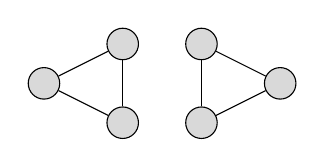
\begin{tikzpicture}[x=1cm,y=1cm] 
				\begin{scope}[scale=1.0]
				
				\tikzstyle{mycircle}=[circle,
				draw=black,
				fill=gray,
				fill opacity = 0.3,
				text opacity=1,
				inner sep=0pt,
				minimum size=4mm,
				font=\small
				]
				\tikzstyle{mycirclewhite}=[circle,
				draw=black,
				text opacity=1,
				inner sep=0pt,
				minimum size=4mm,
				font=\small
				]
				
				\coordinate (pa1) at (0, 0.5);
				\coordinate (pa2) at (1, 0);
				\coordinate (pa3) at (1, 1);
				
				\coordinate (pb1) at (2, 0);
				\coordinate (pb2) at (3, 0.5);
				\coordinate (pb3) at (2, 1);		
				
				\node[mycircle] (a1) at (pa1) {};
				\node[mycircle] (a2) at (pa2) {};
				\node[mycircle] (a3) at (pa3) {};
				
				\node[mycircle] (b1) at (pb1) {};
				\node[mycircle] (b2) at (pb2) {};
				\node[mycircle] (b3) at (pb3) {};		
				
				\draw[-] (a1) -- (a2);
				\draw[-] (a2) -- (a3);
				\draw[-] (a3) -- (a1);
				
				\draw[-] (b1) -- (b2);
				\draw[-] (b2) -- (b3);
				\draw[-] (b3) -- (b1);
				
				\end{scope}
				\end{tikzpicture}
				\caption{$G_1$ - Two disconnected circles, each of length three.}	
				\label{fig:counterExampleWLCai0}
			\end{figure}
		\end{minipage}
		\begin{minipage}{.45\textwidth} % Cai Example 2
			\begin{figure}[H]
				\centering
				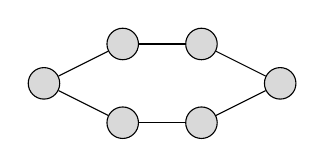
\begin{tikzpicture}[x=1cm,y=1cm] 
				\begin{scope}[scale=1.0]
				
				\tikzstyle{mycircle}=[circle,
				draw=black,
				fill=gray,
				fill opacity = 0.3,
				text opacity=1,
				inner sep=0pt,
				minimum size=4mm,
				font=\small
				]
				\tikzstyle{mycirclewhite}=[circle,
				draw=black,
				text opacity=1,
				inner sep=0pt,
				minimum size=4mm,
				font=\small
				]
				
				\coordinate (pa1) at (0, 0.5);
				\coordinate (pa2) at (1, 0);
				\coordinate (pa3) at (2, 0);		
				\coordinate (pa4) at (3, 0.5);
				\coordinate (pa5) at (2, 1);
				\coordinate (pa6) at (1, 1);		
				
				\node[mycircle] (a1) at (pa1) {};
				\node[mycircle] (a2) at (pa2) {};
				\node[mycircle] (a3) at (pa3) {};		
				\node[mycircle] (a4) at (pa4) {};
				\node[mycircle] (a5) at (pa5) {};
				\node[mycircle] (a6) at (pa6) {};		
				
				\draw[-] (a1) -- (a2);
				\draw[-] (a2) -- (a3);
				\draw[-] (a3) -- (a4);
				\draw[-] (a4) -- (a5);
				\draw[-] (a5) -- (a6);
				\draw[-] (a6) -- (a1);
				
				\end{scope}
				\end{tikzpicture}
				\caption{$G_2$ - A circle of length six.}	
				\label{fig:counterExampleWLCai1}
			\end{figure}		
		\end{minipage}

	\subsubsection{Weisfeiler-Leman Labeling Tree} \label{subsubsec:def_WLLT}
				
		The method is based on the hierarchy of the WL-labels which are constructed by the $1$-dimensional WL-labeling scheme (see algorithm \ref{alg:WLlabeling}).
		This hierarchy can be represented by a hierarchy tree, which we call \textbf{Weisfeiler-Leman labeling tree} (\textbf{WLLT}).
		The WLLT is used in the l-WWLLT method to organize and distinguishing between representations for graphs in a given dataset.
		
		In order to construct a WLLT, we require $D>0$ iterations of WL-labelings on a non-empty database of graphs $\mathcal{G}$.
		Labeled and un-labeled graphs can be treated in the same way, by considering vertex labels as the zeroth WL-labels.
		A WLLT is a rooted tree $T$, where the root is an artificial label. 
		The $i$-th layer of $T$ consists of all WL-labels arising in iteration $i$ of the labeling in any graph in $\mathcal{G}$.
		That is, there exists an edge $(l,l^\prime)$ in $T$ between vertices $l$ and $l^\prime$ if there exists a vertex $v\in V(G)$ in some graph $G\in\mathcal{G}$ and $i\in\IN$ with $l=\ell_i(v)$ and $l^\prime=\ell_{i+1}(v)$.
		The complete construction of the WLLT is sketched in algorithm \ref{alg:WLLTconstruction}.
		
		\begin{algorithm}[H]
			\caption{WLLT construction} \label{alg:WLLTconstruction} 
			\begin{tabbing}
				\textbf{Output:} \= \kill 
				\textbf{Input:} \>a graph dataset $\mathcal{G}$,\\
				\>WL-labelings $\ell_0, \dots \ell_D$ up to depth $D$.\\
				\textbf{Output:} \>WLLT $T$ of height $k$ (unweighted).
			\end{tabbing}	
			\begin{algorithmic}[1]		
				\State Initialize the WLLT as a single root $T=({r}, \emptyset)$
				\For {$G$ in $\mathcal{G}$}
					\For {$i=0$ to $D$}
						\For {$l\in \{ \ell_i(v) | \ v\in V(G) \}$}
							\If {$l\notin T$}
								\State $V(T) = V(T) \cup \{ l \}$
								\State $E(T) = E(T) \cup (p, l)$ where $\ell_{i-1}(v)=p$ and $\ell_{i}(v)=l$ 
							\EndIf					
						\EndFor
					\EndFor
				\EndFor
				\State \textbf{return} $T$
			\end{algorithmic}
		\end{algorithm}
		
		The $i$-th WL-label of vertex $v$ is given by $\ell_i(u)$.		
		Recall, that we use $\Sigma_i$ to denote the set of WL-labels of iteration $i$.
		This set relates to the $i$-th layer $T$.		
		
		Notice that if two vertices have different WL-labels in one refinement step, this implies that they have different WL-labels in all later refinement steps~\cite{1968_Weisfeiler_CONF, 2016_Kriege_NIPS}.
		For a proof by contradiction assume that two WL-labels for two vertices $v$ and $w$ in iteration $j$ are equal ($\ell_j(v) = \ell_j(w)$), but different in any previous iteration $i<j$ ($\ell_i(v) \neq \ell_i(w)$).
		Without loss of generality, say $i$ is maximal and $j$ minimal in this property and thus $i = j-1$.
		But now it is:
		\begin{flalign*}
			\ell_j(v)  &=	 \operatorname{hash}\big(\ell_{j-1}(v),\:\mset{\ell_{j-1}(n)| \ n\in\mathcal{N}_G(v)\:} \big)\\
					   &\neq \operatorname{hash}\big(\ell_{j-1}(w),  \mset{\ell_{j-1}(n)| \ n\in\mathcal{N}_G(w)} \big) &&\text{since }\ell_{j-1}(v)\neq \ell_{j-1}(w)\\
					   &= \ell_j(w)
		\end{flalign*}
		This implies that $\ell_j(v)\neq \ell_j(v)$, which contradicts the assumptions.		
		\[ \forall u,v \in V \ \forall i\in \IN: \quad \ell_k(u)\neq \ell_k(v) \implies \ell_{k+1}(u)\neq \ell_{k+1}(v) \]
		
		\begin{figure}[H]	% Three Graphs and their WL-labels
			\centering
			\begin{tikzpicture}[xscale=0.8, yscale=0.9]
			\centering
			\foreach \shiftamount/\step in {(0,0)/1, (4,0)/2, (8,0)/3}{
				\begin{scope}[shift={\shiftamount}, scale=.80]
				
				\tikzstyle{mycircle}=[circle,
				draw=black,
				fill=white,
				fill opacity=0.4,
				text opacity=1,
				inner sep=0pt,
				minimum size=4mm,
				font=\small
				]	
				
				\coordinate (ptitle) at (1, 0);
				\coordinate (pG1) at (-1.5, 7.5);
				\coordinate (pG2) at (-1.5, 4.5);
				\coordinate (pG3) at (-1.5, 1.5);
				
				\node[rectangle] (title) at (ptitle) {k=\step};
				
				\ifthenelse{\step=1}{
					\node[rectangle] (G1) at (pG1) {$G_1$};
					\node[rectangle] (G2) at (pG2) {$G_2$};
					\node[rectangle] (G3) at (pG3) {$G_3$};
				}
				
				\coordinate (pa1) at (0, 7);
				\coordinate (pa2) at (1, 8);
				\coordinate (pa3) at (2, 7);
				
				\coordinate (pb1) at (0, 4);
				\coordinate (pb2) at (0.5, 5);
				\coordinate (pb3) at (1.5, 5);
				\coordinate (pb4) at (2, 4);
				
				\coordinate (pc1) at (0, 1);
				\coordinate (pc2) at (1, 2);
				\coordinate (pc3) at (2, 2);
				\coordinate (pc4) at (2, 1);		
				
				\node[mycircle] (a1) at (pa1) {};
				\node[mycircle] (a2) at (pa2) {};
				\node[mycircle] (a3) at (pa3) {};
				
				\node[mycircle] (b1) at (pb1) {};
				\node[mycircle] (b2) at (pb2) {};
				\node[mycircle] (b3) at (pb3) {};		
				\node[mycircle] (b4) at (pb4) {};	
				
				\node[mycircle] (c1) at (pc1) {};
				\node[mycircle] (c2) at (pc2) {};
				\node[mycircle] (c3) at (pc3) {};		
				\node[mycircle] (c4) at (pc4) {};	
				
				\path[draw] (a1) -- (a2) -- (a3);
				\path[draw] (b1) -- (b2) -- (b3) -- (b4);
				\path[draw] (c3) -- (c2) -- (c4) -- (c1) -- (c2);
				
				\ifthenelse{\step=2}{		
					\node[mycircle, fill=green]  (a1) at (pa1) {$1$};
					\node[mycircle, fill=blue]   (a2) at (pa2) {$2$};
					\node[mycircle, fill=green]  (a3) at (pa3) {$1$};
					
					\node[mycircle, fill=green]  (b1) at (pb1) {$1$};
					\node[mycircle, fill=blue]   (b2) at (pb2) {$2$};
					\node[mycircle, fill=blue]   (b3) at (pb3) {$2$};		
					\node[mycircle, fill=green]  (b4) at (pb4) {$1$};	
					
					\node[mycircle, fill=blue]   (c1) at (pc1) {$2$};
					\node[mycircle, fill=yellow] (c2) at (pc2) {$3$};
					\node[mycircle, fill=green]  (c3) at (pc3) {$1$};		
					\node[mycircle, fill=blue]   (c4) at (pc4) {$2$};
				}{}
				\ifthenelse{\step=3}{		
					\node[mycircle, fill=red]    (a1) at (pa1) {$4$};
					\node[mycircle, fill=pink] (a2) at (pa2) {$6$};
					\node[mycircle, fill=red]    (a3) at (pa3) {$4$};
					
					\node[mycircle, fill=red]    (b1) at (pb1) {$4$};
					\node[mycircle, fill=violet] (b2) at (pb2) {$7$};
					\node[mycircle, fill=violet] (b3) at (pb3) {$7$};		
					\node[mycircle, fill=red]    (b4) at (pb4) {$4$};	
					
					\node[mycircle, fill=brown] (c1) at (pc1) {$8$};
					\node[mycircle, fill=lime]  (c2) at (pc2) {$9$};
					\node[mycircle, fill=gray]  (c3) at (pc3) {$5$};		
					\node[mycircle, fill=brown] (c4) at (pc4) {$8$};
				}{}	
				%		red, green, blue, cyan, magenta, yellow, black, gray, darkgray, lightgray, brown, lime, olive, orange, pink, purple, teal, violet and white
				\end{scope}	
			}		
			\end{tikzpicture}
			\caption{Examplary WL-labeling on three graphs.}	
			\label{fig:WLlabelingscheme}
		\end{figure}
				
		\begin{figure}[H]
			\centering
			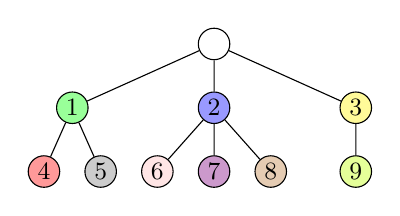
\begin{tikzpicture}[xscale=0.8, yscale=0.9]	
				\begin{scope}[scale=.90]
				
				\tikzstyle{mycircle}=[circle,
				draw=black,
				fill=white,
				fill opacity=0.4,
				text opacity=1,
				inner sep=0pt,
				minimum size=4mm,
				font=\small
				]	
				
				\coordinate (pt01) at (3, 2);
				
				\coordinate (pt11) at (0.5, 1);
				\coordinate (pt12) at (3, 1);
				\coordinate (pt13) at (5.5, 1);
				
				\coordinate (pt21) at (0, 0);
				\coordinate (pt22) at (1, 0);
				\coordinate (pt23) at (2, 0);
				\coordinate (pt24) at (3, 0);
				\coordinate (pt25) at (4, 0);
				\coordinate (pt26) at (5.5, 0);	
				
				\node[mycircle] (t01) at (pt01) {};
				
				\node[mycircle, fill=green]  (t11) at (pt11) {$1$};
				\node[mycircle, fill=blue]   (t12) at (pt12) {$2$};
				\node[mycircle, fill=yellow] (t13) at (pt13) {$3$};
				
				\node[mycircle, fill=red]    (t21) at (pt21) {$4$};
				\node[mycircle, fill=gray]   (t22) at (pt22) {$5$};
				\node[mycircle, fill=pink]   (t23) at (pt23) {$6$};
				\node[mycircle, fill=violet] (t24) at (pt24) {$7$};
				\node[mycircle, fill=brown]  (t25) at (pt25) {$8$};
				\node[mycircle, fill=lime]   (t26) at (pt26) {$9$};
				
				\path[draw] (t11) -- (t01) -- (t12);
				\path[draw] (t13) -- (t01);
				
				\path[draw] (t21) -- (t11) -- (t22);
				\path[draw] (t23) -- (t12) -- (t24);
				\path[draw] (t25) -- (t12);
				\path[draw] (t26) -- (t13);
				
				%		red, green, blue, cyan, magenta, yellow, black, gray, darkgray, lightgray, brown, lime, olive, orange, pink, purple, teal, violet and white
				\end{scope}
			\end{tikzpicture}
			\caption{WLLT to the graphs in figure \ref{fig:WLlabelingscheme}.}
			\label{fig:WLLT}
		\end{figure}
		\begin{figure}[H]
			\centering
			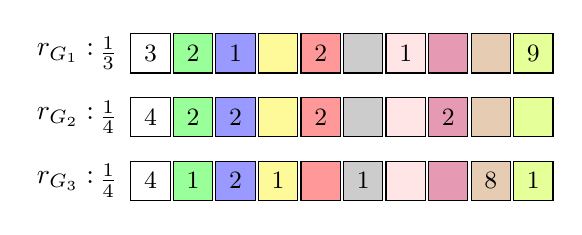
\begin{tikzpicture}[xscale=0.6, yscale=0.9]	
				\begin{scope}[scale=.90]
				
				\tikzstyle{mybox}=[rectangle,
				draw=black,
				fill=white,
				fill opacity=0.4,
				text opacity=1,
				inner sep=0pt,
				minimum size=5mm,
				font=\small
				]	
				
				\coordinate (pg1) at (0, 2); \coordinate (pf1) at (1, 2);
				\coordinate (pg2) at (0, 1); \coordinate (pf2) at (1, 1);
				\coordinate (pg3) at (0, 0); \coordinate (pf3) at (1, 0);
				
				\coordinate (pg1l0) at (2,  2);
				\coordinate (pg1l1) at (3,  2);
				\coordinate (pg1l2) at (4,  2);
				\coordinate (pg1l3) at (5,  2);
				\coordinate (pg1l4) at (6,  2);
				\coordinate (pg1l5) at (7,  2);
				\coordinate (pg1l6) at (8,  2);
				\coordinate (pg1l7) at (9,  2);
				\coordinate (pg1l8) at (10, 2);
				\coordinate (pg1l9) at (11, 2);
				
				\coordinate (pg2l0) at (2,  1);
				\coordinate (pg2l1) at (3,  1);
				\coordinate (pg2l2) at (4,  1);
				\coordinate (pg2l3) at (5,  1);
				\coordinate (pg2l4) at (6,  1);
				\coordinate (pg2l5) at (7,  1);
				\coordinate (pg2l6) at (8,  1);
				\coordinate (pg2l7) at (9,  1);
				\coordinate (pg2l8) at (10, 1);
				\coordinate (pg2l9) at (11, 1);
				
				\coordinate (pg3l0) at (2,  0);
				\coordinate (pg3l1) at (3,  0);
				\coordinate (pg3l2) at (4,  0);
				\coordinate (pg3l3) at (5,  0);
				\coordinate (pg3l4) at (6,  0);
				\coordinate (pg3l5) at (7,  0);
				\coordinate (pg3l6) at (8,  0);
				\coordinate (pg3l7) at (9,  0);
				\coordinate (pg3l8) at (10, 0);
				\coordinate (pg3l9) at (11, 0);
				
				\node (g1) at (pg1) {$r_{G_1}:$}; \node (gf1) at (pf1) {$\frac{1}{3}$};
				
				\node[mybox, fill=white]  (g1l0) at (pg1l0) {$3$};
				
				\node[mybox, fill=green]  (g1l1) at (pg1l1) {$2$};
				\node[mybox, fill=blue]   (g1l2) at (pg1l2) {$1$};
				\node[mybox, fill=yellow] (g1l3) at (pg1l3) {};
				
				\node[mybox, fill=red] 		(g1l4) at (pg1l4) {$2$};
				\node[mybox, fill=gray] 	(g1l5) at (pg1l5) {};
				\node[mybox, fill=pink] 	(g1l6) at (pg1l6) {$1$};
				\node[mybox, fill=purple] 	(g1l7) at (pg1l7) {};
				\node[mybox, fill=brown] 	(g1l8) at (pg1l8) {};
				\node[mybox, fill=lime] 	(g1l9) at (pg1l9) {$9$};
				
				\node (g2) at (pg2) {$r_{G_2}:$}; \node (gf2) at (pf2) {$\frac{1}{4}$};
				
				\node[mybox, fill=white]  (g2l0) at (pg2l0) {$4$};
				
				\node[mybox, fill=green]  (g2l1) at (pg2l1) {$2$};
				\node[mybox, fill=blue]   (g2l2) at (pg2l2) {$2$};
				\node[mybox, fill=yellow] (g2l3) at (pg2l3) {};
				
				\node[mybox, fill=red]    (g2l4) at (pg2l4) {$2$};
				\node[mybox, fill=gray]   (g2l5) at (pg2l5) {};
				\node[mybox, fill=pink]   (g2l6) at (pg2l6) {};
				\node[mybox, fill=purple] (g2l7) at (pg2l7) {$2$};
				\node[mybox, fill=brown]  (g2l8) at (pg2l8) {};
				\node[mybox, fill=lime]   (g2l9) at (pg2l9) {};
				
				
				\node (g3) at (pg3) {$r_{G_3}:$}; \node (gf3) at (pf3) {$\frac{1}{4}$};
				
				\node[mybox, fill=white]  (g3l0) at (pg3l0) {$4$};
				
				\node[mybox, fill=green]  (g3l1) at (pg3l1) {$1$};
				\node[mybox, fill=blue]   (g3l2) at (pg3l2) {$2$};
				\node[mybox, fill=yellow] (g3l3) at (pg3l3) {$1$};
				
				\node[mybox, fill=red]    (g3l4) at (pg3l4) {};
				\node[mybox, fill=gray]   (g3l5) at (pg3l5) {$1$};
				\node[mybox, fill=pink]   (g3l6) at (pg3l6) {};
				\node[mybox, fill=purple] (g3l7) at (pg3l7) {};
				\node[mybox, fill=brown]  (g3l8) at (pg3l8) {$8$};
				\node[mybox, fill=lime]   (g3l9) at (pg3l9) {$1$};
				
				%		red, green, blue, cyan, magenta, yellow, black, gray, darkgray, lightgray, brown, lime, olive, orange, pink, purple, teal, violet and white
				\end{scope}
			\end{tikzpicture}
			\caption{Graph representations of the graphs in figure \ref{fig:WLlabelingscheme}\\with respect to the WLLT in figure \ref{fig:WLLT}.}
			\label{fig:GraphRepresentations}
		\end{figure}
		
		In this thesis, we restrict ourselves to the case that the given graph dataset contains labeled graphs.
		The set of these initial labels can be interpreted as zeroth WL-labels and the set of the vertices of the first layer in a corresponding WLLT ($\Sigma_0$).
		Notice that these have depth $1$ in the WLLT and further layers of depth $D$ correspond to the D-1-th WL-labeling.
		
		Figures \ref{fig:plotwlltl2e0aids2915h-25m} and \ref{fig:plotwlltmutagl2} display two examples of WLLTs.
		Both examples display the tree for depth $D=2$, and thus with two layers.
		Notice, how the much bigger and diverse dataset AIDS generates a much bigger tree than the dataset MUTAG with the same number of WL-labeling iterations.
		
		As mentioned before, the l-WWLLT method aims to define meaningful distances between the WL-labels in the WLLT by adjusting weights on its edges.		
		An example of a weighted WLLT is shown in figure \ref{fig:plotwlltmutagl2weighted}.
		The edge colors and edge lengths correspond to the edge weights.
		
		\begin{figure}[H]
			\centering
			\begin{subfigure}{0.49\textwidth}
				\centering
				\includegraphics[width=1.0\linewidth]{images/plot_wllt_MUTAGl2}
				\caption{Example WLLT: MUTAG, $d=2$.}
				\label{fig:plotwlltmutagl2}
			\end{subfigure}
			\begin{subfigure}{0.49\textwidth}
				\centering
				\includegraphics[width=1.0\linewidth]{images/plot_wllt_l2_e0_AIDS_29_15h-25m}
				\caption{Example WLLT: AIDS, $d=2$.}
				\label{fig:plotwlltl2e0aids2915h-25m}
			\end{subfigure}
			\caption{Unweighted WLLT examples}\label{fig:combined}
		\end{figure}
		
		\begin{figure}[H]
			\centering
			\includegraphics[width=0.7\linewidth]{images/plot_wllt_MUTAGl2_weighted}
			\caption{Weighted WLLT example: AIDS, $d=2$.}
			\label{fig:plotwlltmutagl2weighted}
		\end{figure}
		
		\paragraph{Runtime of the WLLT Construction}	
		As shown in section \ref{subsubsec:def_WLlabeling}, the computation of $d$ iterations of WL-labels for a graph with $m$ edges can be done in $\mathcal{O}(dm)$.
		Using non-negative integers as WL-labels allows for an easy construction of the WL-label hierarchy (parent list) in linear time.
		The definition of edge weights requires to initialize $p$ values, if the WLLT holds $p$ many WL-labels and the (possibly artificial) root.
		Depending on the desired initialization, the edge weights can be defined during the construction.
		For a more sophisticated initialization note, we may limit $p$ by the number of WL iterations, and the total number of vertices in the whole graph dataset.
		A stricter limitation of $p$ is not useful, if the initialization method is not specified.		
		Thus we conclude that for a graph dataset $\mathcal{G}$ of $N$ graphs with at most $m$ edges, the WLLT can be constructed with uniform weights in $\mathcal{O}(Ndm)$.
		
\subsection{Kernels} \label{subsec:def_kernels}

	A function $f:\IR\to\IC$ is called \textbf{positive-definite} if for any real numbers $x_1,\dots, x_n$ the matrix 
	$A = [a_{i,j}]^n_{i,j=1}$ with $a_{i,j} = f(x_i-x_j)$ is positive \textbf{semi-definite}, that is $x^\intercal A x \ge 0$ for all $x\in\IR^n$.
	In case of a symmetric matrix, this implies that it is positive definite if all its eigenvalues are non-negative.
	If it further is $x^\intercal A x = 0$ only for $0=x\in\IR^n$, the matrix is called \textbf{strictly positive definite}~\cite{2008_Hofmann_CONF}. %Other definitions: 2019_Togninalli_NIPS - Appendix A1
	A function $f$ is (\textbf{strictly}) \textbf{negative-definite} if $-f$ is (strictly) positive-definite~\cite{2007_Borgwardt_BOOK}.	
		
	Kernels are similarity functions that can be interpreted as a dot product in a high-dimensional space.
	They are often used in learning algorithms that rely on dot products, such as classifications tasks using support vector machines (SVMs)~\cite{2002_Scholkopf_CONF, 2019_Togninalli_NIPS}.
	Other applications are regression~\cite{1996_Drucker_CONF}, clustering~\cite{1996_Vapnik_CONF} and principal component analysis~\cite{1997_Schoelkopf_CONF}.
	
	Formally, a \textbf{kernel} on a set $X$ is a function $k:X\times X \to\IR$ such that there is a (reproducing) real Hilbert space $\mathcal{H}$ and a mapping $\phi:X\to\mathcal{H}$ (feature map) such that $k(x,y) = \langle \phi(x), \phi(y) \rangle_\mathcal{H}$ for all $x, y\in X$~\cite{1999_Haussler_CONF, 2008_Hofmann_CONF}. 
	Here, $\langle \cdot,\cdot \rangle_\mathcal{H}$ denotes the inner product of $\mathcal{H}$.
	The definition of definiteness extends from matrices to kernels, in terms of the Gram matrix or kernel matrix $K:=\big[ k(x, y) \big]_{x, y}$~\cite{2008_Hofmann_CONF}.
	Equivalently, a function $k:X\times X\to\IR$ is a kernel if and only if for every subset $\{x_1, \dots, x_n\}\subseteq X$ the matrix $\big[k(x_i, x_j)\big]^n_{i,j=1}$ is positive semi-definite~\cite{2016_Kriege_NIPS, 2019_Togninalli_NIPS}.
	$\big[k(x_i, x_j)\big]^n_{i,j=1}$ is called \textbf{Gram matrix} of $k$ with respect to $x_1, \dots, x_n$.
	Or in other words a symmetric function $k:X\times X\to\IR$ is called a positive definite kernel, if
	\begin{equation} \label{eq:pd_kernel}
		\forall c_i\in\IR \; \forall n\in\IN \; \forall x_i\in X:\qquad \sum_{i,j=1}^{n} c_i c_j k(x_i, x_j) \ge 0
	\end{equation}
	With respect to kernel a kernel function $k$ we call it \textbf{conditional positive definite}, if it satisfies equation \ref{eq:pd_kernel} for all $c_i\in\IR$ with $\sum_{i=1}^{n} c_i = 0$~\cite{2019_Togninalli_NIPS}.
	The \textbf{Dirac Kernel} $k_{\delta}$ is defined by $k_{\delta}(x,y)=1$, if $x=y$ and $0$ otherwise.
	
	A \textbf{graph kernel} on a set of graphs $\mathcal{G}$ is a symmetric, positive semidefinite kernel $k:\mathcal{G}\times \mathcal{G}\to \IR$ with domain $\mathcal{G}$.
	Notice that graph kernels can be defined on both the vertices or the edges of a graph~\cite{2008_Hofmann_CONF} and in general do not need to be positive (semi-)definite.	
	But if they are, one can use the so-called kernel trick, by representing the computation as an inner product in a any Hilbert space.
	This is most useful for high dimensional feature spaces, since the explicit computation for associated feature maps usually involves high costs~\cite{2003_Gaertner_CONF}.
	However for example the Optimal Assignment Kernel proved useful, despite being not positive definite in general (see ~\cite{2005_Froehlich_ICML})~\cite{2018_Vert_CONF}.
	
	\subsubsection{Laplacian Kernel} \label{subsec:def_LaplacianKernel}
		
		The \textbf{Laplacian Kernel} has favorable conditions for positive definiteness in the case of non-Euclidean distances~\cite{1984_Berg_BOOK, 2015_Feragen_IEEE}, and when using noiseless data~\cite{2015_Rupp_CONF}.
		Since many graph similarity measure, as well as the l-WWLLT distance, may not be an Euclidean distance, this kernel is useful to derive a kernel from such a proposed graph similarity measure.
		It is defined as:		
		\begin{equation}\label{eq:LaplacianKernel}
		k(x,y) = \exp\big( -\lambda d(x,y) \big)
		\end{equation}
		\citeauthor{1938_Schoenberg_CONF} showed that the Laplacian Kernel is positive definite for all $0<\lambda\in\IR$, if and only if the ground distance $d$ is (conditional) negative definite.
		For a proof of this claim see \cite{1938_Schoenberg_CONF} and Theorem C.3.2 in \cite{2017_Bollobas_BOOK}.
	
	\subsubsection{Tree-sliced Wasserstein Kernel} \label{sec:def_TSWKernel}
	
		Recall equation \ref{eq:TreeWassDist} for the definition of the negative definite Tree Wasserstein Distance.
		\citeauthor{2019_Le_NIPS} proposed a the \textbf{Tree-sliced Wasserstein Distance} % Definition 1. page 4
		\begin{equation} \label{eq:TreeSlicedWassersteinDistance}
			\text{TSW}(\mu, \nu) := \frac{1}{n}\sum_{i=1}^{n}\mathbb{W}_{d_{T_i}}(\mu, \nu)
		\end{equation}
		Using it in the Laplacian kernel (equation \ref{eq:LaplacianKernel}) results in the \textbf{Tree-sliced-Wasserstein} (\textbf{TSW}) \textbf{Kernel} $k_{\text{TSW}}$~\cite{2019_Le_NIPS}:
		\[ k_{\text{TSW}}(\mu, \nu) := \exp\big( -\lambda \text{TSW}(\mu, \nu) \big) \]
		
		Since we define the l-WWLLT as an instance of the Tree-sliced Wasserstein Kernel, it is important to notice that this kernel is positive definite.		
		As mentioned in section \ref{subsec:def_LaplacianKernel}, the Laplacian kernel is positive definite for all $\lambda>0$, if and only if the ground distance $d$ is (conditional) negative definite.		
		This in turn highly depends on the used ground metric.
		For example, Wasserstein distances with discrete metrics as ground distances are conditional negative definite~\cite{2018_Gardner_IEEE}. 		
		\citeauthor{2019_Le_NIPS} showed that the Tree Wasserstein distance is negative definite (Proposition 2 in ~\cite{2019_Le_NIPS} following~\cite{1984_Berg_BOOK} on pages 66-67), 		
		and thus also conditionally negative definite.
		Since the Tree-sliced Wasserstein Distance is thus a sum of negative definite functions, it is negative definite itself and the TSW Kernel is positive definite as desired.
		
	% WL Graph Kernels - 2011_Shervashidze_JMLR
	\subsubsection{Weisfeiler-Leman Graph Kernel} \label{subsec:def_WLkernel}
		For $d$ iterations of the WL-labeling scheme, lets call a graph $G$ with the WL-labeling of the $i$-th iteration the \textbf{WL graph at depth} $i$:
		\[ G_i = (V,E,l_i) \]
		Furthermore lets define the \textbf{WL-sequence up to height $i$} of set graph $G$ as the sequence:
		\[ ( G_0,G_1,\dots,G_i ) \ = \ ( (V,E,\ell_0),(V,E,\ell_1), \dots,(V,E,\ell_i) ) \]
		As said before, we consider the original labels of a graph $G=(V,E,L)$ as labels of the zeroth WL iteration ($L=\ell_0$).
		
		Let $k$ be any positive semi-definite kernel on two graphs $G$ and $H$. 
		Then the \textbf{Weisfeiler-Leman} (\textbf{WL}) \textbf{Graph Kernel}~\cite{2011_Shervashidze_JMLR} with $D$ iterations with $k$ as base kernel is defined as
		\[ k_{\text{WL}}^{(D)}(G, H) \ = \sum_{i=0}^{D} k(G_i,H_i) \]
		A more general definition can be derived, when weighting the WL iterations with $0\le \alpha_i\in \IR$:
		\[ k_{\text{WL}}^{(D)}(G, H) \ = \sum_{i=0}^{D} \alpha_i k(G_i,H_i) \]
		This weight function allows for example to emphasize larger substructures, which are represented by WL-labels from deeper WL iterations~\cite{2021_Schulz_CONF}.
	
%		\paragraph{Weisfeiler-Leman Subtree Graph Kernel} %LaterTODO GENERAL kernel From where comes the first definition?
%		Again let $G$ and $H$ be two graphs.
%		Recall, that in this thesis we define the WL-labels, such that all $\Sigma_i$ are pairwise disjoint.
%		We require this property in the following definition.
%		Define for every $i$, $\Sigma_i=(\sigma_{i,1},\dots,\sigma_{i|\Sigma_i|})$ as the ordered tuple of the set $\Sigma_i$.
%		Define a map $c_i: \{G, H\}\times \Sigma_i\to\IN$ such that $c_i(G,\sigma_{i,j})$ is the number of occurrences of the WL label $\sigma_{i,j}$ in the graph $G$.
%		The \textbf{Weisfeiler-Leman Subtree} (\textbf{WLST}) \textbf{Graph Kernel} on $G$ and $H$ for $D$ WL-labeling iterations is defined as:
%		\[ k_{\text{WLST}}^{(d)}(G,H) \ = \ \langle \psi_{\text{WLST}}^{(d)}(G), \psi_{\text{WLST}}^{(d)}(H) \rangle \]
%		where \[ \psi_{\text{WLST}}^{(d)}(G) = \big( c_0(G,\sigma_{0,1}),\dots, c_0(G,\sigma_{0,|\Sigma_0| }),\dots,c_h(G,\sigma_{h,1}),\dots, c_h(G,\sigma_{h,|\Sigma_h| }) \big) \]
%		In other words, the WLST Kernel counts the common (original and) WL-labels in the two graphs.
%		%Note that due to the runtime of algorithm \ref{alg:WeisfeilerLemanEmbedding}, one can compute the WL-Subtree Kernel in $\mathcal{O}(dm)$.
%		
%		One can show that the WL Kernel and the WLST Kernel are closely related.
%		Let $k$ be a function to count pairs of matching vertex labels in two graphs:
%		\[ k(G,H) := \sum_{v\in V(G)}\sum_{w\in V(H)} \delta\big( \ell(v), \ell(w) \big) \]
%		Then $k_{\text{WL}}^{(d)}(G,H) = k_{\text{WLST}}^{(d)}(G,H)$. %LaterTODO: Prove?
%		
%		Let $\mathcal{G}$ be a set of graphs and $\Theta_i$ a set of hard clustering functions (i.e. partitionings) of the set of depth-$i$ unfolding trees $\mathcal{T}^{(i)}$ appearing in the graphs in $\mathcal{G}$.
%		Regard each element of $\Theta_i$ as a function $\rho:\mathcal{T}:\Sigma_i\to [k]$, where $k$ is the number of clusters defined by $\rho$.
%		Then, for any graphs $G, H\in\mathcal{G}$ and depth parameter $d\in\IN$, the \textbf{relaxed Weisfeiler-Leman Subtree} (R-WLST) \textbf{Kernel}~\cite{2021_Schulz_CONF} is defined as:
%		\[ k^d_{\text{R-WLST}}(G,H) = \sum\limits_{i=0,\dots, d}\sum\limits_{\rho\in\Theta_i}\sum\limits_{v\in V(G)}\sum\limits_{w\in V(H)} \delta\Big( \rho\big( T^i(G,v)\big),\; \rho\big( T^i(H,w)\big) \Big) \]
%		$k^d_{\text{R-WLST}}$ is positive semi-definite and equivalent to the original WL-Subtree Kernel for $\Theta_i=\{\rho_i\}$. %LaterTODO: prove
	
	% WL-OA - 2016_Kriege_NIPS
	\subsubsection{Weisfeiler-Leman Optimal Assignment Graph Kernel} \label{subsec:def_WLOA}
		The \textbf{Weisfeiler-Leman Optimal Assignment} (\textbf{WL-OA}) \textbf{Graph Kernel} proposed by \citeauthor{2016_Kriege_NIPS} is similarly based on the hierarchy implied by the WL-labels~\cite{2016_Kriege_NIPS}.		
		To understand the difference to the approach in this thesis, we briefly summarize the definition of the WL-OA.
		Consider two graphs $G$ and $H$ and their vertex sets $V(G)$, $V(H) \subseteq\mathcal{V}$.
		Let $\mathcal{B}\big(V(G), V(H)\big)$ denote the set of all bijections between $V(G)$, $V(H)$.
		Given $d$ iterations of the WL-labeling scheme for two vertices $v,w\in\mathcal{V}$, define the base kernel of the WL-OA as the sum of equal WL-labels over all these iterations:
		\[ k_d(v,w) := \sum_{i=0}^{d} k_{\delta}\big( \ell^i(v), \ell^i(w) \big) \]
		Now the WL-OA Kernel is defined as
		\[ K(G, H) := K_{\mathcal{B}}^{k}\big( V(G), V(H) \big) = \max\limits_{B\in\mathcal{B}\big(V(G), V(H)\big)} \sum_{(v,w)\in B}k_d(v,w)  \]
		If the vertex sets have different carnality one may introduce artificial vertices $z$ to the smaller set with $k_d(z,x)=0$ for all $x\in\mathcal{V}$.
		
		Notice that $k_d(v,w)$ corresponds to the number of matching WL-labels in the refinement sequence.
		As mentioned before, if two vertices have different WL-labels at any depth, all their WL-labels in deeper depths are different too.
		Thus the WL-OA Kernel bases its similarity measure on the length of the path in the WLLT to the lowest common ancestor of the WL-labelings of two vertices.
						
	% WWL graph kernel - 2019_Togninalli_NIPS
	\subsubsection{Wasserstein Weisfeiler-Leman Graph Kernel} \label{subsec:def_WWLKernel}
		
		Similarly to the WL Graph Kernel (section  \ref{subsec:def_WLkernel}) and the WL-OA Kernel (section \ref{subsec:def_WLOA}), the \textbf{Wasserstein Weisfeiler-Leman} (\textbf{WWL}) \textbf{Graph Kernel} is constructed using WL-labels of a graphs vertices.
		Different is however, that all WL-labels are used.
		Let there be $D$ iterations of the WL-labeling scheme and consider a graph $G=(\{ v_1, \dots, v_n \}, E)$ with $n$ vertices.
		Again let $\Sigma=\IN$ be the set of all possible WL-labels.
		For a vertex $v$ in a graph $G$, define the vertex embedding $f_{\text{WL}}^{D}:V\to\Sigma^{D+1}$ as the (row) vector of all WL-labels, that are assigned to $v$:		
		\[ f_{\text{WL}}^{D}(v) = \big( \ell_0(v), \dots, \ell_D(v) \big)  \]
		Now define a graph representation $f_{\text{WL}}^{D}$ (graph embedding scheme~\cite{2019_Togninalli_NIPS}) as 
		\[ F_{\text{WL}}^{D}(G) = \begin{pmatrix}
		f_{\text{WL}}^{D}(v_1) \\ \dots \\ f_{\text{WL}}^{D}(v_n)
		\end{pmatrix}  = \big( \ell_i(v_j) \big)_{\begin{subarray}{l}
			j\in\{0,\dots,D\}\\
			i\in\{1,\dots,n\}
			\end{subarray}} \in \Sigma^{n\times (D+1)} \]
		Note that \citeauthor{2019_Togninalli_NIPS} described this graph representation as the concatenation of WL features, which are the \textit{column} vectors of all WL-labels for all vertices, in one fixed WL-labeling iteration.
		Next, we define the normalized Hamming distance $d_{\text{Ham}}: \Sigma^{(D+1)} \to \IR$ as the normalized count of equal entries in two vectors:
		\[ d_{\text{Ham}}(f_0, f_1) = \frac{1}{D+1} \sum\limits_{i=0}^{D} \delta(f_0, f_1) \]		
		For $\lambda\in \IR^+$ and using $d_{\text{Ham}}$ as ground metric for the $L^1$-Wasserstein distance (see equation \ref{eq:discreteWassDist}), we can define the WWL Kernel as:		
		\begin{equation} \label{eq:WWLKernel}
			K_{\text{WWL}}(G,H) = \exp(-\lambda \mathcal{W}(F_{\text{WL}}^{D}(G), F_{\text{WL}}^{D}(H)) )
		\end{equation}
		
		Notice, that we define the l-WWLLT distance, very similarly. 
		As ground distance, we use a tree metric, which depends on edge weights in the WLLT, which is changed by a learning process.
		Due to the nature of the used ground distance, we also switch the computation of the Wasserstein distance to the tree-sliced variation (section \ref{subsec:def_WassDist}).

\subsection{Cluster Learning} \label{subsec:def_cl_scores}

	There are many different metrics to evaluate a given clustering.
	Different scores measure the tightness or denseness, separation, and intra and inter dispersion of clusters.
	In general, we prefer clusterings with high separation and inter dispersion and with tight and dense clusters or low intra dispersion.
	We now state definitions of three cluster scores, which were used in the evaluation process.
	
	The \textbf{Silhouette coefficient} (SS) $S_{\text{SC}}$ is based on the comparison of the clusters tightness and separation~\cite{1987_Rousseeuw_ELSEVIER}.
	Let $a$ be the mean intra-cluster distance and $b$ be the distance to the nearest cluster for each sample.
	Then $S_{\text{SC}}$ is defined as
	\[ S_{\text{SC}} := \frac{ b - a }{ \max(a, b) } \quad \in[-1, 1]\]
	That is the mean of the distances between a sample and the nearest cluster that it is not a part of.
	Thus positive values close to $1$ indicate that the data is clustered in \textit{well separated} clusters, and the samples are less similar to the other samples in the assigned cluster, than the to the ones in the closest other cluster.
	Negative values indicate that a sample has been assigned to the wrong cluster, i.a. another cluster is denoted as more similar.
	Values near zero indicate \textit{overlapping clusters} - indicating that samples are cannot reliably be separated from other clusters~\cite{1987_Rousseeuw_ELSEVIER}.
	The used implementation was provided by \textbf{Scikit-Learn.org}.
	\footnote{ \url{https://scikit-learn.org/stable/modules/generated/sklearn.metrics.silhouette_score.html\#sklearn.metrics.silhouette_score},		\url{https://github.com/scikit-learn/scikit-learn/blob/f3f51f9b6/sklearn/metrics/cluster/_unsupervised.py\#L39} }
	
	The \textbf{Davies-Bouldin score} (SDB) $S_{\text{DB}}$ gives an average similarity of each cluster with its most similar cluster~\cite{1979_Davies_IEEE}.
	Let $M_{i,j}$ be the distance between characteristic vectors of cluster $i$ and $j$, and $S_i$ the dispersion of cluster $i$.
	The function
	\[ R_{i,j} := \frac{S_i + S_j}{M_{i,j}} \]
	is a non-negative, symmetric similarity function. 	
	Furthermore, the similarity expressed by $R_{i,j}$ decreases, if the distance $M_{i,j}$ between the clusters increases, while the dispersion of the individual clusters remains constant.
	Now the Davies-Bouldin score $S_{\text{DB}}$ is defined as the average maximum dis-similarity $R_{i,j}$ between all $n$ clusters:
	\[ S_{\text{DB}} := \frac{1}{n}\sum_{i=0}^{n-1}\; \max\limits_{i\neq j} R_{i,j} \] 
	Thus the score is based on the ratio of within-cluster distances to between-cluster distances and clusters which are \textit{farther apart} and \textit{less dispersed} yield a better score.
	Lower (positive) values indicate a better clustering.
	But the score is only zero if the dispersion of both clusters $i$ and $j$ vanish (that is each cluster consists of indistinguishable samples).	
	Note that the dataset must be partitioned into at least two clusters with different cluster centers for the score to have meaning.
	The used implementation was provided by \textbf{Scikit-Learn.org}.
	\footnote{ \url{https://scikit-learn.org/stable/modules/generated/sklearn.metrics.davies_bouldin_score.html},	\url{https://github.com/scikit-learn/scikit-learn/blob/f3f51f9b6/sklearn/metrics/cluster/_unsupervised.py\#L307} }
	
	The \textbf{Calinski-Harabasz score} (SCH) $S_{\text{CH}}$ (also known as variance ration criterion) is the ratio of the mean between-cluster (intra) dispersion and the within-cluster (inter) dispersion~\cite{1974_Calinski_CONF}.
	Let $n$ be the size of the dataset and $k\ge 1$ the number of clusters. 
	For cluster $i$ let $C_i$ be the set of data points in it, $c_i$ its the center and $n_i$ its size. Let $c_D$ be the center of the whole dataset.
	Then define the \textit{between group dispersion matrix} as
	\[ B_k := \sum_{i=0}^{k-1} n_i (c_i - c_E) (c_i - c_E)^\intercal \]
	and the \textit{within-cluster dispersion matrix} as
	\[ W_k := \sum_{i=0}^{k-1} \sum_{x \in C_i} (x - c_i) (x - c_i)^\intercal \]
	Now the Calinski-Harabasz score is defined as the 
	\[ S_{\text{CH}} = \frac{\tr\big(B_k\big)}{\tr\big(W_k\big)} \ \frac{n-k}{k-1} \]	
	The score is higher when clusters are \textit{dense} and \textit{well separated}.
	% Also, that score is generally higher for convex clusters than other concepts of clusters, such as density based clusters.	
	The used implementation was provided by \textbf{Scikit-Learn.org}.
	\footnote{ \url{https://scikit-learn.org/stable/modules/generated/sklearn.metrics.calinski_harabasz_score.html},	\url{https://github.com/scikit-learn/scikit-learn/blob/f3f51f9b6/sklearn/metrics/cluster/_unsupervised.py\#L253} }
